\chapter{Problematik und Lösungsansätze}

Über die vergangenen Jahre haben es Smartphones unter Endverbrauchern zu enormer Beliebtheit geschafft und sind mittlerweile überall im Alltag in Gebrauch(Real Challanges in Mobile App Development (X)). Mit dem Smartphone werden Urlaube geplant, Kinokarten gekauft, Rechnungen bezahlt. Wir benutzen das Smartphone und seine Anwendungen um mit Dienstleistern zu kommunizieren(Challenges and Opportunities of mob app dev (X)). Diese Allgegenwart von Smartphones hat entsprechend die Aufmerksamkeit von Software Entwicklern auf sich gezogen. Stand 2013 befanden sich etwa 800.000 mobile Anwendungen in Apple's AppStore, 650.000 im Android Store, 120.000 im Windows Marketplace und 100.000 in Blackberry's AppWorld(Real Challanges in Mobile App Development (X)). Die rasante Entwicklung sieht man, wenn man diese Zahlen mit dem Stand 2016 vergleicht: etwa 2.000.000 Anwendungen befinden sich in Apple's AppStore und in Androids Google Play sogar mehr als 2.560.000\footcite{StatistikApps}. Wie in oben genannter Statistik bereits erkennbar, gibt es mehrere Handelsplattformen mit jeweils einem eigenen Betriebssystem, Entwicklerwerkzeuge und Bibliotheken, wie zum Beispiel Android, iOS, Windows Phone oder BlackBerry. Fast jährlich erscheinen für diese Betriebssysteme Major Releases(Challenges and Opportunities of mob app dev (X)). Diese Fragmentierung der Plattformen und Standards führen auf der einen Seite zu verstärktem Wettkampf, was sich positiv auf Fortschritt und Weiterentwicklung auswirkt. Auf der anderen Seite ist dies eine Barriere in der Entwicklung von Inhalten und Services, was die Benutzer an eine spezifische Technologie bindet oder Entwicklerunternehmen einen Mehraufwand bereitet, um ihre Services auf mehreren Plattformen zu anzubieten(Challenges for Mobile Application Dev (X)). 
\\
\\
Die Charakteristiken von mobilen Anwendungen und die Erwartungen der Benutzer führen zu folgender Basisherausforderung in der mobilen Anwendungsentwicklung: 'Liefere schnell aus und reagiere schnell auf Feedback', und dies in einem nicht endenden Zyklus. Jedes Unternehmen, dessen mobile Anwendungen 1-Stern Bewertungen und Kommentare mit Adjektiven  wie 'verwirrend', 'unvollständig' oder 'langsam' bekommt, wird auf dem Markt verlieren, wenn diese Kritiken nicht ernst genommen und schnell Verbesserungen implementiert werden(Challenges and Opportunities of mob app dev (X)). 
\\
\\
Die 3 großen Kategorien in der mobilen Anwendungsentwicklung sind nativ, Web-basiert und hybrid. Native Anwendungen sind für ein spezifisches Betriebssystem entwickelt und nutzen dessen Schnittstellen und Bibliotheken direkt. Sie müssen für jedes Betriebssystem auf dem sie laufen sollen separat entwickelt werden. Web-basierte Anwendungen laufen in einem Web Browser, der auf dem Smartphone installiert sein muss. Hybride Anwendungen sind 'native-wrapped' Web-Anwendungen. Bei nativen Anwendungen können, im Gegensatz zu Web-basierten Anwendungen, alle nativen Funktionen des Endgeräts genutzt werden, wie zum Beispiel Kameras und Sensoren(Challenges and Opportunities of mob app dev (X)). 
\\
\\
Hybride und Cross-Plattform Anwendungen versuchen den Vorteil der Plattformunabhängigkeit Web-basierter Anwendungen mit dem Vorteil des Nutzens nativer Funktionen von nativen Anwendungen zu vereinen. Diese Form von Anwendungsentwicklung erzielt weltweit immer mehr Popularität aufgrund der Tatsache, dass sich ihr Code auf mehreren Plattformen kompilieren lässt. Entwicklungswerkzeuge für hybride und Cross-Plattform Anwendungsentwicklung basieren meist auf Programmiersprachen aus der Webentwicklung wie zum Beispiel HyperTest Markup Language (HTML), JavaScript oder Cascading Style Sheets (CSS). Dazu kommt dann eine Art Wrapper-Code für die Zugriffe auf die nativen Schnittstellen (APIs). Auf diese Weise können dann auch die nativen Funktionen wie Kameras und Sensoren angesprochen werden. Diese Form von Anwendungsentwicklung verspricht eine Reduzierung der Entwicklungskosten bei neuen Anwendungen, was sie für Entwicklerunternehmen attraktiv macht(Comparison of Cross-Platform Mobile Development (X)). Die Arbeit von X und Y (Comparison of Cross-Platform Mobile Development(X)) hat allerdings auch ergeben, dass ein gravierender Nachteil hybrider Anwendungen im Gegensatz zu nativen Anwendungen die Performance ist. Aus diesem Grund beschäftigt sich diese Arbeit mit dem Vergleich verschiedener Frameworks, die für Entwicklung hybrider und Cross-Plattform Anwendungen angeboten werden. Ein besonderes Augenmerk wird dabei auch auf die Performance bei der Nutzung nativer Funktionen im Vergleich zur nativen Anwendung gelegt.
\\
\\
In den letzten Jahren wurden einige Arbeiten über mobile Anwendungsentwicklung und auch Cross-Plattform, beziehungsweise hybride Anwendungsentwicklung veröffentlicht. In der Arbeit von X und Y (Comparison of Cross-Platform Mobile Development(X)) von 2012 wurden die 4 Frameworks Rhodes, PhoneGap, DragonRad and MoSync miteinander verglichen. Bei ihrer Arbeit konnten sie folgende Vorteile bei der hybriden Anwendungsentwicklung ausmachen: 

\begin{itemize}
\item Reduzierung der benötigten Skills: Hybride Frameworks verwenden meist gängige Programmiersprachen wie HTML oder JavaScript.
\item Weniger Code: Da plattformübergreifender Code produziert wird, muss nicht mehr für jede Plattform eine eigene komplette Anwendung mit separater Codebase entwickelt werden.
\item Reduzierung der Entwicklungszeit und Wartungskosten, da nur eine Anwendung entwickelt und gewartet werden muss im Vergleich zu mehreren nativen Anwendungen. 
\item Die Entwickler müssen sich in weniger APIs einarbeiten und sich auskennen, da nicht direkt mit den APIs der Plattformen gearbeitet wird, sondern mit der API des jeweiligen Framework.
\item Wachsende Marktanteile für das Business hinter der Anwendung. 
\end{itemize}

Zusammengefasst lässt sich sagen, dass die hybride Anwendungsentwicklung einerseits verspricht die Investitionskosten zu senken und andererseits den Verkauf der Anwendungen auf mehrere Märkte ausweitet. Die Bewertungskriterien, anhand derer X und Y die Frameworks in ihrer Arbeit evaluiert haben, waren folgende: 

\begin{itemize}
\item Die Betriebssysteme, die von den Frameworks unterstützt werden
\item Lizenzen für die Frameworks zur Evaluierung der Geschäftsbedingungen
\item Verfügbare Programmiersprachen für die Entwicklung der Anwendungen
\item Verfügbarkeit der APIs hinsichtlich der Fragestellungen welche nativen Funktionen genutzt werden können
\item die Architektur, die für den Entwicklungsprozess der Anwendung zur Verfügung steht
\item Integrated Development Environments (IDEs) die verfügbar und nutzbar sind
\end{itemize}

Für die API-Tests hat sich für die 4 von X und Y ausgewählten Frameworks folgendes Bild ergeben(Abbildung \ref{fig:Ergebnis_API_Test_Publ}): 

\begin{figure}[h]
	\centering
	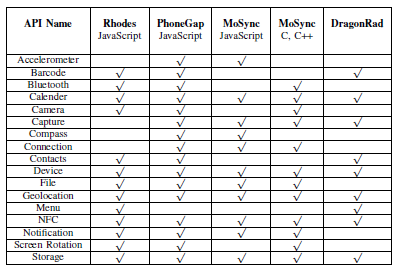
\includegraphics[width=0.7\textwidth]{Bilder/Ergebnis_Sensornutzung_Comparison_of_Cross-Platform_Mob_Dev.PNG}
	\caption{Ergebnis API-Tests aus X und Y Arbeit: Comparison of Cross-Platform Mobile Development aus 2012}
	\label{fig:Ergebnis_API_Test_Publ}
\end{figure}

Wie man in Abbildung \ref{fig:Ergebnis_API_Test_Publ} erkennen kann, schafft es vor allem PhoneGAp alle bis auf eine getestete native Funktionalität umzusetzen. Allerdings fanden X und Y heraus, dass vor allem die Frameworks, welche auf JavaScript basieren, deutliche Performance-Probleme haben. Aus diesem Grund raten die Autoren davon ab JavaScript-basierte Frameworks für Anwendungen mit komplexen Funktionalitäten oder im Hintergrund laufende Services zu nutzen. Auch sei die Unterstützung von High-End Grafiken und 3D-Technologien unzureichend. 
\\
\\
Eine weitere Arbeit, die sich mit dem Vergleich von hybriden Frameworks beschäftigt hat ist die von X und Y: Cross-Platform Mobile Development: A Study on Apps with Animations(X) aus dem Jahr 2014. Die Frameworks, die in dieser Arbeit evaluiert wurden sind MoSync, Titanium, JQuery \& JQuery Mobile und PhoneGap. Die Bewertungskriterien, die die Autoren aufstellten sind folgende:

\begin{itemize}
\item Lizenzmodell und Kosten
\item Die Vielfältigkeit und Qualität der verfügbaren APIs
\item Das Angebot an Tutorials
\item Die Größe der Community
\item Die Komplexität des Codes um die vorgegebene Anwendung zu implementieren
\item Die Benutzerfreundlichkeit der IDE des Frameworks
\item Die Liste der unterstützten Geräte
\item Inwieweit die Frameworks das Erstellen einer nativen Benutzeroberfläche unterstützen 
\item Das geforderte Basiswissen im Bereich Programmierung und Technologiekenntnis für jedes Framework
\end{itemize}

Wie man an den Bewertungskriterien oben schon erkennen kann, gaben die Autoren eine Beispiel-Anwendung vor, die mit Hilfe der 4 ausgewählten Frameworks implementiert wurde, um diese gegeneinander zu evaluieren. Um einem Bias entgegenzuwirken wurden für die einzelnen Entwicklungen Entwickler ausgewählt, die mit der jeweiligen Programmiersprache bereits vertraut waren. Die Frameworks wurden anschließend in den oben aufgeführten Kategorien mit Noten von 0 (schlecht) bis 5 (sehr gut) bewertet. Unten stehende Tabelle (Abbildung (X)) zeigt die Ergebnisse:

 \begin{figure}[h]
	\centering
	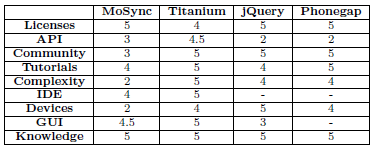
\includegraphics[width=0.65\textwidth]{Bilder/Ergebnis_Framework_Bewertung_Publ_2.PNG}
	\caption{Ergebnis Framework Evaluation von X und Y: Cross-Platform Mobile Development: A Study on Apps with Animations aus 2014}
	\label{fig:Ergebnis_API_Test_Publ}
\end{figure}

Auf Basis oben (Abbildung (X)) dargestellten Ergebnisses bewerten die Autoren das Framework Titanium als das Bestes unter den getesteten für Anwendungen mit Animationen. Begründung hierfür ist, dass Titanium Animationen und Übergangseffekte nativ unterstützt und die Performance gut ist und vermuten lässt, dass auch bei komplexeren Anwendungen die Performance noch ausreichend sein wird. 
\\
\\
In dieser Arbeit sollen ebenfalls, wie bei oben vorgestellten Publikationen, hybride Frameworks direkt miteinander verglichen werden. Um die zu evaluierenden Frameworks auszuwählen, wird zunächst eine Marktanalyse durchgeführt, welche anzeigen soll, welche Frameworks die aktuell attraktivsten sind. Für die Evaluation wird eine Test-Anwendung entwickelt, die mit den ausgewählten Frameworks implementiert werden soll. Diese Anwendung wird zuvor noch als Referenz für zum Beispiel die Performance noch nativ implementiert. Die Anzahl der Frameworks, die mit dieser Anwendung getestet werden ist dabei auf 5 limitiert. Allerdings werden noch weitere Frameworks mit in die Evaluation aufgenommen. Diese können aber nur nach Bewertungskriterien verglichen werden, die nicht direkt mit dem Entwicklungsprozess zusammenhängen. Es wird versucht die Kriterienkataloge der oben vorgestellten Publikationen mittels einer Umfrage unter Anwendungsentwicklern noch zu erweitern. Da aufgrund bisheriger Publikationen davon auszugehen ist, dass es nicht 'das eine' Framework für alle Problemstellungen gibt, soll das Ergebnis dieser Arbeit ein Entscheidungsbaum werden, anhand dessen das ideale Framework je Problematik ermittelt werden kann. 

